\begin{figure}
  \caption{From \textcite{Novy-Marx2012}, ``Marginal strategy performance''. Comparison of returns, standard deviation and Sharpe ratio of long top-decile/short bottom-decile of lagged performance strategies, varying the lag}
  \label{fig:NovyMarx2012_Fig1}
  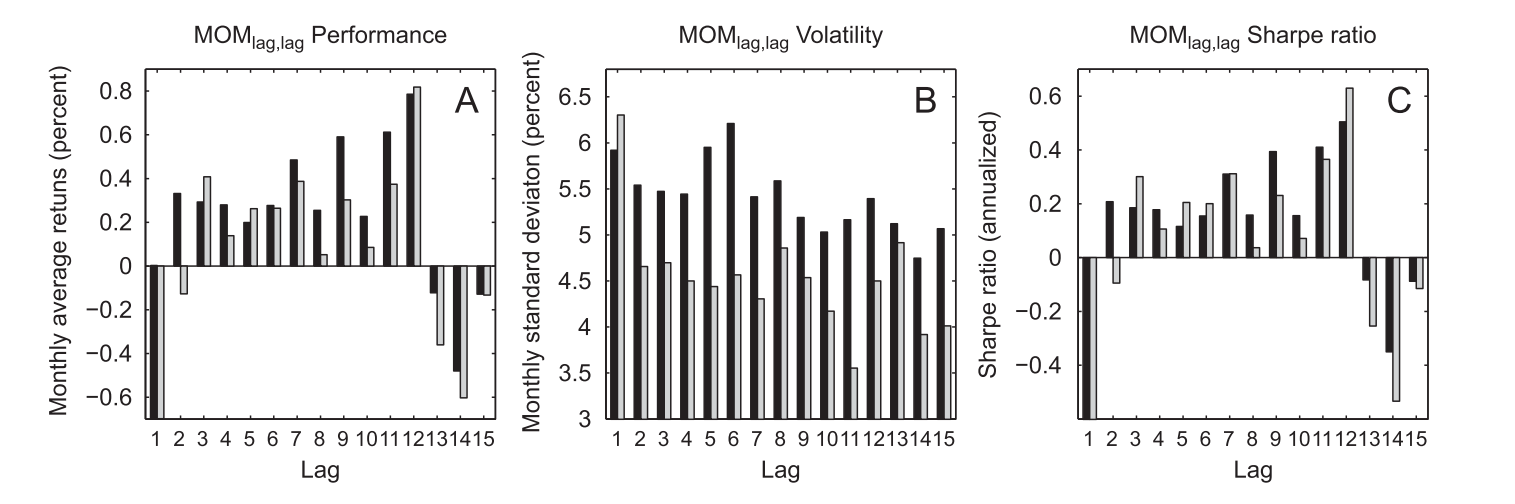
\includegraphics[width=\linewidth]{Figures/NovyMarx2012_Fig1_better.png}
  Description from original paper:
  \begin{quote}
  \textit{Fig. 1. Marginal strategy performance. This figures shows the average monthly returns (Panel A), monthly standard deviations (Panel B) and annual Sharpe ratio (Panel C) to winners-minus-losers strategies. Winners and losers are defined as the top and bottom deciles of performance in a single month, respectively, starting lag months prior to portfolio formation. Dark bars show value-weighted results and light bars show equal-weighted results. Average monthly returns for the one month reversals are $-1.04$\% (value-weighted) and $-2.82$\% (equal-weighted). The sample covers April 1927 to December 2010.}  
  \end{quote}
\end{figure}
